\chapter{Исследовательская часть}

В данном разделе будут приведены примеры работы программ, постановка эксперимента и сравнительный анализ алгоритмов на основе полученных данных.

\section{Технические характеристики}

Технические характеристики устройства, на котором выполнялось исследование.

\begin{enumerate}
	\item Операционная система: Windows 10 Корпоративная, Версия	21H1, Сборка ОС 19043.2006.
	\item Память: 8 ГБ.
	\item Процессор: AMD Ryzen 5 4600H с видеокартой Radeon Graphics \\3.00 ГГц \cite{processor}.
\end{enumerate}

Исследование проводилось на ноутбуке, включенном в сеть электропитания. Во время исследования ноутбук был нагружен только встроенными приложениями окружения, а также непосредственно системой.

\section{Демонстрация работы программы}

На рисунках \ref{fig:democl}, \ref{fig:demov}, \ref{fig:demo} представлены результаты работы реализаций алгоритмов.

\captionsetup{justification=centering,singlelinecheck=false}

\begin{figure}[H]
	\centering
	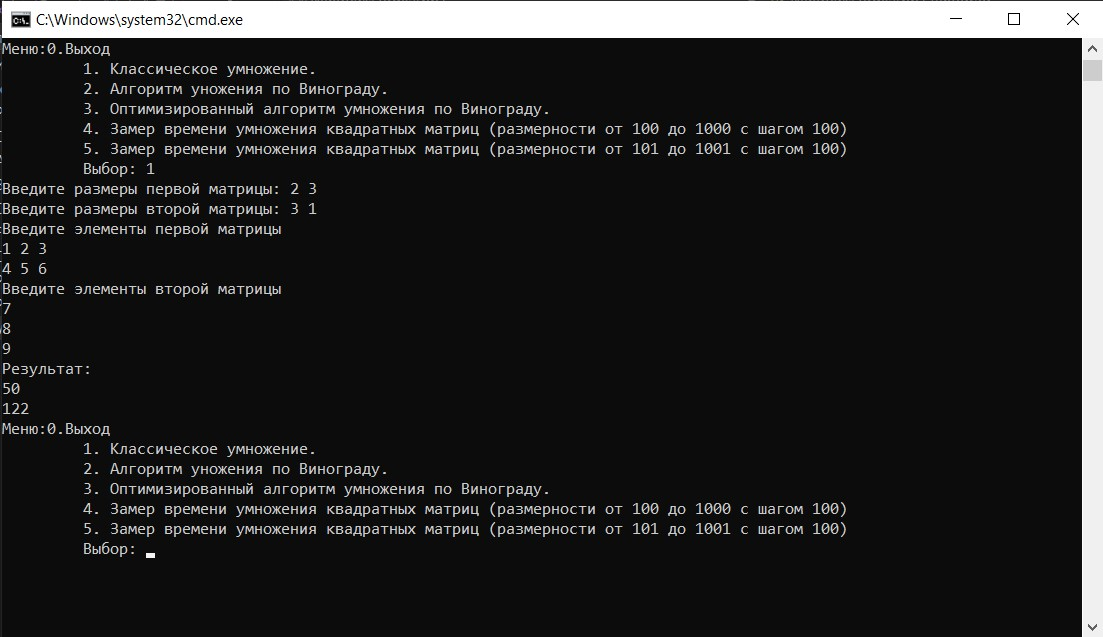
\includegraphics[width=1\linewidth]{inc/img/democl}
	\caption{Демонстрация корректной работы реализации классического алгоритма умножения матриц}
	\label{fig:democl}
\end{figure}
\begin{figure}[H]
	\centering
	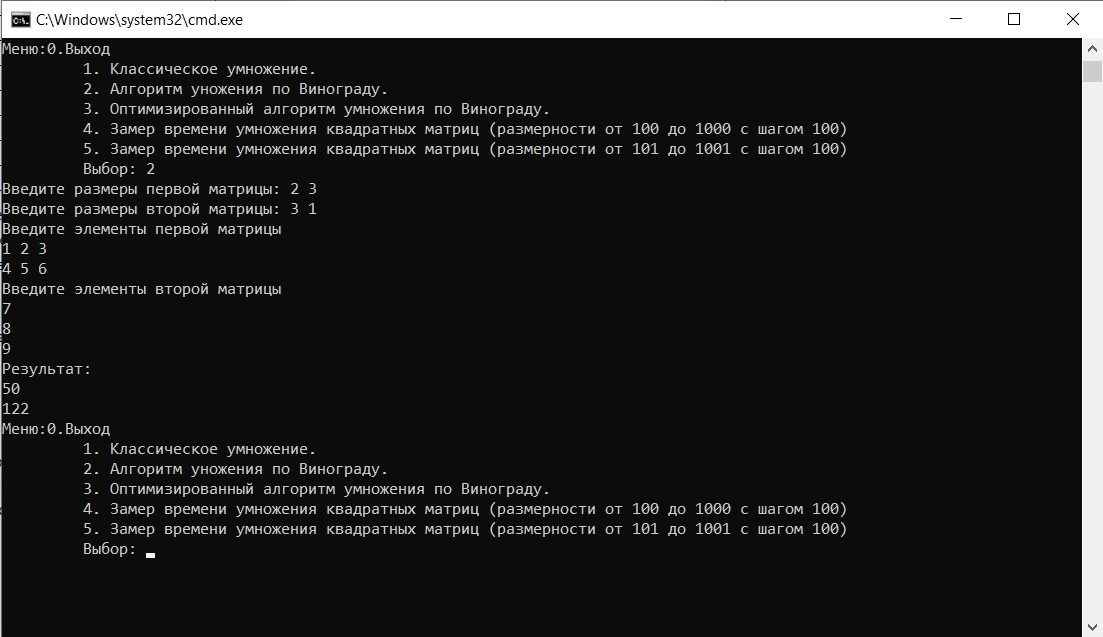
\includegraphics[width=1\linewidth]{inc/img/demov}
	\caption{Демонстрация корректной работы реализации алгоритма Винограда}
	\label{fig:demov}
\end{figure}

\begin{figure}[H]
	\centering
	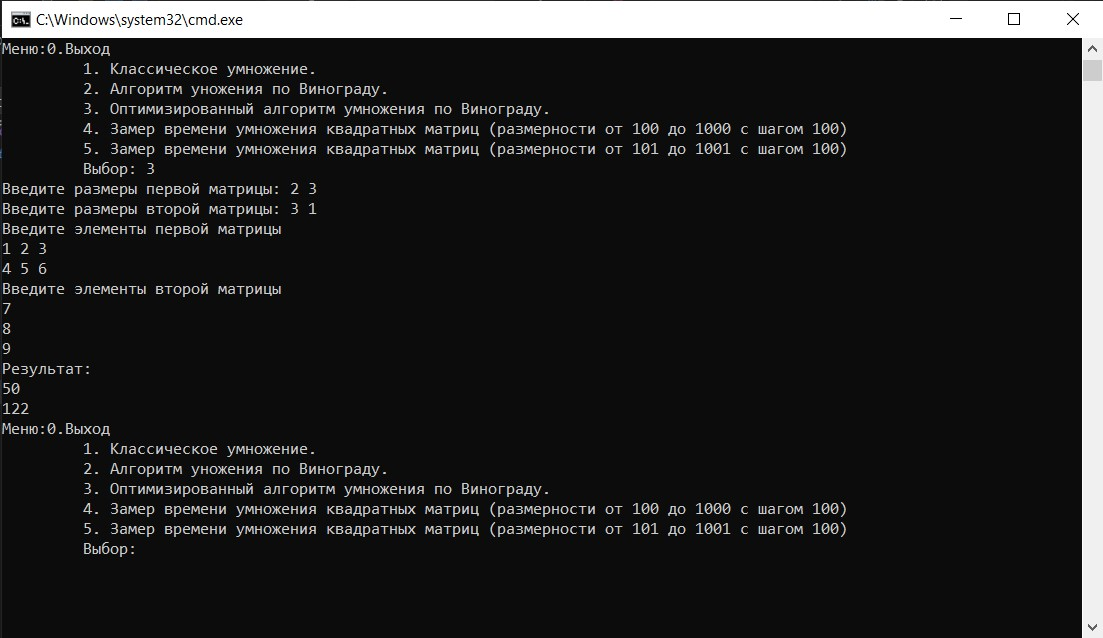
\includegraphics[width=1\linewidth]{inc/img/demo}
	\caption{Демонстрация корректной работы реализации оптимизированного алгоритма Винограда}
	\label{fig:demo}
\end{figure}



\section{Время выполнения реализаций алгоритмов}

Время выполнения реализаций алгоритмов было замерено при помощи функции clock() \cite{cpplangtime}. Данная функция всегда возвращает значения времени, а именно сумму системного и пользовательского процессорного времени текущего процесса, значения типа float --- время в тиках.

Замеры времени для каждой длины массива проводились 100 раз. В качестве результата взято среднее время работы алгоритма на данном размере матрицы.



\section{Сравнение времени выполнения реализаций алгоритмов}
Для сравнения времени работы алгоритмов умножения матриц были использованы квадратные матрицы размером от 100 до 1000 с шагом 100. Эксперимент для более точного результата повторялся 100 раз. Итоговый результат рассчитывался как средний из полученных результатов. Результаты измерений показаны в таблице \ref{tbl:even} и на рисунке \ref{fig:even}.
\captionsetup{justification=raggedright,singlelinecheck=false}
\begin{table}[H]
	\begin{center}
		\caption{Время работы алгоритмов сортировки на отсортированных данных (тики)}
		\label{tbl:even}
		\begin{tabular}{|c|c|c|c|}
			\hline
			Размер & Classic &  Vinograd &  Optimized Vinograd \\
			\hline
			100&	4,6&	4,4&	3,1\\
			\hline
			200&	35,5&	34,5&	23,9\\
			\hline
			300&	119,3&	115,7&	80\\
			\hline
			400&	286,5&	276,7&	195,7\\
			\hline
			500&	578,2&	538,7&	404,6\\
			\hline
			600&	955,1&	935,2&	700,8\\
			\hline
			700&	1588,1&	1488,5&	1115,8\\
			\hline
			800&	2663,8&	2254,7&	2060,6\\
			\hline
			900&	3584,3&	3348,4&	3033,1\\
			\hline
			1000&	5246&	5006,7&	3747,1\\
			\hline
		\end{tabular}
	\end{center}
	
\end{table}

\captionsetup{justification=centering,singlelinecheck=false}

\begin{figure}[H]
	\centering
	\includegraphics[width=1\linewidth]{"inc/img/Снимок экрана 2022-10-20 014553"}
	\caption{Зависимость времени работы алгоритма от размера (четного) матрицы (время в тиках)}
	\label{fig:even}
\end{figure}
%TODO переделать выводы

Из результатов экспериментов можно сделать вывод о том, что алгоритм Винограда эффективнее по времени чем классический алгоритм умножения матриц в среднем на 7\%. Оптимизированный алгоритм работает быстрее обычного алгоритма Винограда.

Для сравнения времени работы алгоритмов умножения матриц были использованы квадратные матрицы размером от 101 до 1001 с шагом 100. Эксперимент для более точного результата повторялся 100 раз. Итоговый результат рассчитывался как средний из полученных результатов. Результаты измерений показаны в таблице \ref{tbl:odd} и на рисунке \ref{fig:odd}.
\captionsetup{justification=raggedright,singlelinecheck=false}
\begin{table}[H]
	\begin{center}
		\caption{Время работы реализаций алгоритмов умножения матриц при нечетных размерах (тики)}
		\label{tbl:odd}
		\begin{tabular}{|c|c|c|c|}
			\hline
			Размер & Classic &  Vinograd &  Optimized Vinograd \\
			\hline
			101&	4,7&	4,7&	3,5\\
			\hline
			201&	35,9&	35,3&	26,1\\
			\hline
			301&	120,1&	116,8&	87,2\\
			\hline
			401&	283,6&	277,27&	206,6\\
			\hline
			501&	555,6&	543&	406,4\\
			\hline
			601&	987,8&	931,2&	693,1\\
			\hline
			701&	1559,6&	1470,9&	1096,2\\
			\hline
			801&	2373,9&	2194,1&	1631,4\\
			\hline
			901&	3496,1&	3173,9&	2354,7\\
			\hline
			1001&	4966,4&	4670,1&	3452,7\\
			\hline
		\end{tabular}
	\end{center}
	
\end{table}

\captionsetup{justification=centering, singlelinecheck=false}

\begin{figure}[H]
	\centering
	\includegraphics[width=1\linewidth]{"inc/img/Снимок экрана 2022-10-20 011917"}
	\caption{Зависимость времени работы алгоритма от размера (нечетного) матрицы (время в тиках)}
	\label{fig:odd}
\end{figure}

Для случая с нечётными размерами матриц можно сделать те же выводы, что и для случая с чётными. При этом можно заметить, что классический алгоритм в среднем работает за то же время, что и при чётных размерах, в то время как алгоритм Винограда и его оптимизация работают дольше за счёт дополнительных операций при нечётном случае. 

\section*{Вывод}

Алгоритм Винограда эффективнее по времени чем классический, но требует дополнительную память.


